
%% bare_jrnl_transmag.tex
%% V1.4a
%% 2014/09/17
%% by Michael Shell
%% see http://www.michaelshell.org/
%% for current contact information.
%%
%% This is a skeleton file demonstrating the use of IEEEtran.cls
%% (requires IEEEtran.cls version 1.8a or later) with an IEEE 
%% Transactions on Magnetics journal paper.
%%
%% Support sites:
%% http://www.michaelshell.org/tex/ieeetran/
%% http://www.ctan.org/tex-archive/macros/latex/contrib/IEEEtran/
%% and
%% http://www.ieee.org/

%%*************************************************************************
%% Legal Notice:
%% This code is offered as-is without any warranty either expressed or
%% implied; without even the implied warranty of MERCHANTABILITY or
%% FITNESS FOR A PARTICULAR PURPOSE! 
%% User assumes all risk.
%% In no event shall IEEE or any contributor to this code be liable for
%% any damages or losses, including, but not limited to, incidental,
%% consequential, or any other damages, resulting from the use or misuse
%% of any information contained here.
%%
%% All comments are the opinions of their respective authors and are not
%% necessarily endorsed by the IEEE.
%%
%% This work is distributed under the LaTeX Project Public License (LPPL)
%% ( http://www.latex-project.org/ ) version 1.3, and may be freely used,
%% distributed and modified. A copy of the LPPL, version 1.3, is included
%% in the base LaTeX documentation of all distributions of LaTeX released
%% 2003/12/01 or later.
%% Retain all contribution notices and credits.
%% ** Modified files should be clearly indicated as such, including  **
%% ** renaming them and changing author support contact information. **
%%
%% File list of work: IEEEtran.cls, IEEEtran_HOWTO.pdf, bare_adv.tex,
%%                    bare_conf.tex, bare_jrnl.tex, bare_conf_compsoc.tex,
%%                    bare_jrnl_compsoc.tex, bare_jrnl_transmag.tex
%%*************************************************************************


% *** Authors should verify (and, if needed, correct) their LaTeX system  ***
% *** with the testflow diagnostic prior to trusting their LaTeX platform ***
% *** with production work. IEEE's font choices and paper sizes can       ***
% *** trigger bugs that do not appear when using other class files.       ***                          ***
% The testflow support page is at:
% http://www.michaelshell.org/tex/testflow/



\documentclass[journal,transmag]{IEEEtran}
%
% If IEEEtran.cls has not been installed into the LaTeX system files,
% manually specify the path to it like:
% \documentclass[journal]{../sty/IEEEtran}





% Some very useful LaTeX packages include:
% (uncomment the ones you want to load)


% *** MISC UTILITY PACKAGES ***
%
%\usepackage{ifpdf}
% Heiko Oberdiek's ifpdf.sty is very useful if you need conditional
% compilation based on whether the output is pdf or dvi.
% usage:
% \ifpdf
%   % pdf code
% \else
%   % dvi code
% \fi
% The latest version of ifpdf.sty can be obtained from:
% http://www.ctan.org/tex-archive/macros/latex/contrib/oberdiek/
% Also, note that IEEEtran.cls V1.7 and later provides a builtin
% \ifCLASSINFOpdf conditional that works the same way.
% When switching from latex to pdflatex and vice-versa, the compiler may
% have to be run twice to clear warning/error messages.






% *** CITATION PACKAGES ***
%
%\usepackage{cite}
% cite.sty was written by Donald Arseneau
% V1.6 and later of IEEEtran pre-defines the format of the cite.sty package
% \cite{} output to follow that of IEEE. Loading the cite package will
% result in citation numbers being automatically sorted and properly
% "compressed/ranged". e.g., [1], [9], [2], [7], [5], [6] without using
% cite.sty will become [1], [2], [5]--[7], [9] using cite.sty. cite.sty's
% \cite will automatically add leading space, if needed. Use cite.sty's
% noadjust option (cite.sty V3.8 and later) if you want to turn this off
% such as if a citation ever needs to be enclosed in parenthesis.
% cite.sty is already installed on most LaTeX systems. Be sure and use
% version 5.0 (2009-03-20) and later if using hyperref.sty.
% The latest version can be obtained at:
% http://www.ctan.org/tex-archive/macros/latex/contrib/cite/
% The documentation is contained in the cite.sty file itself.






% *** GRAPHICS RELATED PACKAGES ***
%
\ifCLASSINFOpdf
  \usepackage[pdftex]{graphicx}
  % declare the path(s) where your graphic files are
  % \graphicspath{{../pdf/}{../jpeg/}}
  % and their extensions so you won't have to specify these with
  % every instance of \includegraphics
  % \DeclareGraphicsExtensions{.pdf,.jpeg,.png}
\else
  % or other class option (dvipsone, dvipdf, if not using dvips). graphicx
  % will default to the driver specified in the system graphics.cfg if no
  % driver is specified.
  % \usepackage[dvips]{graphicx}
  % declare the path(s) where your graphic files are
  % \graphicspath{{../eps/}}
  % and their extensions so you won't have to specify these with
  % every instance of \includegraphics
  % \DeclareGraphicsExtensions{.eps}
\fi
% graphicx was written by David Carlisle and Sebastian Rahtz. It is
% required if you want graphics, photos, etc. graphicx.sty is already
% installed on most LaTeX systems. The latest version and documentation
% can be obtained at: 
% http://www.ctan.org/tex-archive/macros/latex/required/graphics/
% Another good source of documentation is "Using Imported Graphics in
% LaTeX2e" by Keith Reckdahl which can be found at:
% http://www.ctan.org/tex-archive/info/epslatex/
%
% latex, and pdflatex in dvi mode, support graphics in encapsulated
% postscript (.eps) format. pdflatex in pdf mode supports graphics
% in .pdf, .jpeg, .png and .mps (metapost) formats. Users should ensure
% that all non-photo figures use a vector format (.eps, .pdf, .mps) and
% not a bitmapped formats (.jpeg, .png). IEEE frowns on bitmapped formats
% which can result in "jaggedy"/blurry rendering of lines and letters as
% well as large increases in file sizes.
%
% You can find documentation about the pdfTeX application at:
% http://www.tug.org/applications/pdftex




% *** MATH PACKAGES ***
%
%\usepackage[cmex10]{amsmath}
% A popular package from the American Mathematical Society that provides
% many useful and powerful commands for dealing with mathematics. If using
% it, be sure to load this package with the cmex10 option to ensure that
% only type 1 fonts will utilized at all point sizes. Without this option,
% it is possible that some math symbols, particularly those within
% footnotes, will be rendered in bitmap form which will result in a
% document that can not be IEEE Xplore compliant!
%
% Also, note that the amsmath package sets \interdisplaylinepenalty to 10000
% thus preventing page breaks from occurring within multiline equations. Use:
%\interdisplaylinepenalty=2500
% after loading amsmath to restore such page breaks as IEEEtran.cls normally
% does. amsmath.sty is already installed on most LaTeX systems. The latest
% version and documentation can be obtained at:
% http://www.ctan.org/tex-archive/macros/latex/required/amslatex/math/





% *** SPECIALIZED LIST PACKAGES ***
%
%\usepackage{algorithmic}
% algorithmic.sty was written by Peter Williams and Rogerio Brito.
% This package provides an algorithmic environment fo describing algorithms.
% You can use the algorithmic environment in-text or within a figure
% environment to provide for a floating algorithm. Do NOT use the algorithm
% floating environment provided by algorithm.sty (by the same authors) or
% algorithm2e.sty (by Christophe Fiorio) as IEEE does not use dedicated
% algorithm float types and packages that provide these will not provide
% correct IEEE style captions. The latest version and documentation of
% algorithmic.sty can be obtained at:
% http://www.ctan.org/tex-archive/macros/latex/contrib/algorithms/
% There is also a support site at:
% http://algorithms.berlios.de/index.html
% Also of interest may be the (relatively newer and more customizable)
% algorithmicx.sty package by Szasz Janos:
% http://www.ctan.org/tex-archive/macros/latex/contrib/algorithmicx/




% *** ALIGNMENT PACKAGES ***
%
%\usepackage{array}
% Frank Mittelbach's and David Carlisle's array.sty patches and improves
% the standard LaTeX2e array and tabular environments to provide better
% appearance and additional user controls. As the default LaTeX2e table
% generation code is lacking to the point of almost being broken with
% respect to the quality of the end results, all users are strongly
% advised to use an enhanced (at the very least that provided by array.sty)
% set of table tools. array.sty is already installed on most systems. The
% latest version and documentation can be obtained at:
% http://www.ctan.org/tex-archive/macros/latex/required/tools/


% IEEEtran contains the IEEEeqnarray family of commands that can be used to
% generate multiline equations as well as matrices, tables, etc., of high
% quality.




% *** SUBFIGURE PACKAGES ***
%\ifCLASSOPTIONcompsoc
%  \usepackage[caption=false,font=normalsize,labelfont=sf,textfont=sf]{subfig}
%\else
%  \usepackage[caption=false,font=footnotesize]{subfig}
%\fi
% subfig.sty, written by Steven Douglas Cochran, is the modern replacement
% for subfigure.sty, the latter of which is no longer maintained and is
% incompatible with some LaTeX packages including fixltx2e. However,
% subfig.sty requires and automatically loads Axel Sommerfeldt's caption.sty
% which will override IEEEtran.cls' handling of captions and this will result
% in non-IEEE style figure/table captions. To prevent this problem, be sure
% and invoke subfig.sty's "caption=false" package option (available since
% subfig.sty version 1.3, 2005/06/28) as this is will preserve IEEEtran.cls
% handling of captions.
% Note that the Computer Society format requires a larger sans serif font
% than the serif footnote size font used in traditional IEEE formatting
% and thus the need to invoke different subfig.sty package options depending
% on whether compsoc mode has been enabled.
%
% The latest version and documentation of subfig.sty can be obtained at:
% http://www.ctan.org/tex-archive/macros/latex/contrib/subfig/



% *** FLOAT PACKAGES ***
%
%\usepackage{fixltx2e}
% fixltx2e, the successor to the earlier fix2col.sty, was written by
% Frank Mittelbach and David Carlisle. This package corrects a few problems
% in the LaTeX2e kernel, the most notable of which is that in current
% LaTeX2e releases, the ordering of single and double column floats is not
% guaranteed to be preserved. Thus, an unpatched LaTeX2e can allow a
% single column figure to be placed prior to an earlier double column
% figure. The latest version and documentation can be found at:
% http://www.ctan.org/tex-archive/macros/latex/base/


%\usepackage{stfloats}
% stfloats.sty was written by Sigitas Tolusis. This package gives LaTeX2e
% the ability to do double column floats at the bottom of the page as well
% as the top. (e.g., "\begin{figure*}[!b]" is not normally possible in
% LaTeX2e). It also provides a command:
%\fnbelowfloat
% to enable the placement of footnotes below bottom floats (the standard
% LaTeX2e kernel puts them above bottom floats). This is an invasive package
% which rewrites many portions of the LaTeX2e float routines. It may not work
% with other packages that modify the LaTeX2e float routines. The latest
% version and documentation can be obtained at:
% http://www.ctan.org/tex-archive/macros/latex/contrib/sttools/
% Do not use the stfloats baselinefloat ability as IEEE does not allow
% \baselineskip to stretch. Authors submitting work to the IEEE should note
% that IEEE rarely uses double column equations and that authors should try
% to avoid such use. Do not be tempted to use the cuted.sty or midfloat.sty
% packages (also by Sigitas Tolusis) as IEEE does not format its papers in
% such ways.
% Do not attempt to use stfloats with fixltx2e as they are incompatible.
% Instead, use Morten Hogholm'a dblfloatfix which combines the features
% of both fixltx2e and stfloats:
%
% \usepackage{dblfloatfix}
% The latest version can be found at:
% http://www.ctan.org/tex-archive/macros/latex/contrib/dblfloatfix/




%\ifCLASSOPTIONcaptionsoff
%  \usepackage[nomarkers]{endfloat}
% \let\MYoriglatexcaption\caption
% \renewcommand{\caption}[2][\relax]{\MYoriglatexcaption[#2]{#2}}
%\fi
% endfloat.sty was written by James Darrell McCauley, Jeff Goldberg and 
% Axel Sommerfeldt. This package may be useful when used in conjunction with 
% IEEEtran.cls'  captionsoff option. Some IEEE journals/societies require that
% submissions have lists of figures/tables at the end of the paper and that
% figures/tables without any captions are placed on a page by themselves at
% the end of the document. If needed, the draftcls IEEEtran class option or
% \CLASSINPUTbaselinestretch interface can be used to increase the line
% spacing as well. Be sure and use the nomarkers option of endfloat to
% prevent endfloat from "marking" where the figures would have been placed
% in the text. The two hack lines of code above are a slight modification of
% that suggested by in the endfloat docs (section 8.4.1) to ensure that
% the full captions always appear in the list of figures/tables - even if
% the user used the short optional argument of \caption[]{}.
% IEEE papers do not typically make use of \caption[]'s optional argument,
% so this should not be an issue. A similar trick can be used to disable
% captions of packages such as subfig.sty that lack options to turn off
% the subcaptions:
% For subfig.sty:
% \let\MYorigsubfloat\subfloat
% \renewcommand{\subfloat}[2][\relax]{\MYorigsubfloat[]{#2}}
% However, the above trick will not work if both optional arguments of
% the \subfloat command are used. Furthermore, there needs to be a
% description of each subfigure *somewhere* and endfloat does not add
% subfigure captions to its list of figures. Thus, the best approach is to
% avoid the use of subfigure captions (many IEEE journals avoid them anyway)
% and instead reference/explain all the subfigures within the main caption.
% The latest version of endfloat.sty and its documentation can obtained at:
% http://www.ctan.org/tex-archive/macros/latex/contrib/endfloat/
%
% The IEEEtran \ifCLASSOPTIONcaptionsoff conditional can also be used
% later in the document, say, to conditionally put the References on a 
% page by themselves.




% *** PDF, URL AND HYPERLINK PACKAGES ***
%
\usepackage{url}
% url.sty was written by Donald Arseneau. It provides better support for
% handling and breaking URLs. url.sty is already installed on most LaTeX
% systems. The latest version and documentation can be obtained at:
% http://www.ctan.org/tex-archive/macros/latex/contrib/url/
% Basically, \url{my_url_here}.




% *** Do not adjust lengths that control margins, column widths, etc. ***
% *** Do not use packages that alter fonts (such as pslatex).         ***
% There should be no need to do such things with IEEEtran.cls V1.6 and later.
% (Unless specifically asked to do so by the journal or conference you plan
% to submit to, of course. )

\usepackage{color,soul} % for highlighting only

%http://tex.stackexchange.com/questions/61265/why-doesnt-the-ieeetran-document-class-recognize-definition-environments
\newtheorem{definition}{Definition}

% correct bad hyphenation here
\hyphenation{op-tical net-works semi-conduc-tor}


\begin{document}
%
% paper title
% Titles are generally capitalized except for words such as a, an, and, as,
% at, but, by, for, in, nor, of, on, or, the, to and up, which are usually
% not capitalized unless they are the first or last word of the title.
% Linebreaks \\ can be used within to get better formatting as desired.
% Do not put math or special symbols in the title.
\title{Bare Demo of IEEEtran.cls for \textsc{Transactions on Magnetics}}



% author names and affiliations
% transmag papers use the long conference author name format.

\author{\IEEEauthorblockN{
	J. Kyle Medley\IEEEauthorrefmark{1},
	Jonathan R. Karr\IEEEauthorrefmark{2},
	and Herbert M. Sauro\IEEEauthorrefmark{1}
	}
\IEEEauthorblockA{
	\IEEEauthorrefmark{1}Department of Bioengineering, University of Washington, Seattle WA 98195\\
	\IEEEauthorrefmark{2}Department of Genetics \& Genomic Siences, Icahn School of Medicine at Mount Sinai, New York NY 10029
	}
\thanks{Manuscript received December x, xxxx; revised September x, xxxx.
Corresponding author: J. K. Medley (email: medleyj@uw.edu).}}



% The paper headers
\markboth{IEEE Transactions on Biomedical Engineering,~Vol.~13, No.~9, September~2015}%
{Medley \MakeLowercase{\textit{et al.}}: Bare Demo of IEEEtran.cls for Journals}
% The only time the second header will appear is for the odd numbered pages
% after the title page when using the twoside option.
% 
% *** Note that you probably will NOT want to include the author's ***
% *** name in the headers of peer review papers.                   ***
% You can use \ifCLASSOPTIONpeerreview for conditional compilation here if
% you desire.




% If you want to put a publisher's ID mark on the page you can do it like
% this:
%\IEEEpubid{0000--0000/00\$00.00~\copyright~2014 IEEE}
% Remember, if you use this you must call \IEEEpubidadjcol in the second
% column for its text to clear the IEEEpubid mark.



% use for special paper notices
%\IEEEspecialpapernotice{(Invited Paper)}


% for Transactions on Magnetics papers, we must declare the abstract and
% index terms PRIOR to the title within the \IEEEtitleabstractindextext
% IEEEtran command as these need to go into the title area created by
% \maketitle.
% As a general rule, do not put math, special symbols or citations
% in the abstract or keywords.
\IEEEtitleabstractindextext{%
\begin{abstract}
Lorem ipsum dolor sit amet, consectetur adipiscing elit, sed do eiusmod tempor incididunt ut labore et dolore magna aliqua. Ut enim ad minim veniam, quis nostrud exercitation ullamco laboris nisi ut aliquip ex ea commodo consequat. Duis aute irure dolor in reprehenderit in voluptate velit esse cillum dolore eu fugiat nulla pariatur. Excepteur sint occaecat cupidatat non proident, sunt in culpa qui officia deserunt mollit anim id est laborum.
Lorem ipsum dolor sit amet, consectetur adipiscing elit, sed do eiusmod tempor incididunt ut labore et dolore magna aliqua. Ut enim ad minim veniam, quis nostrud exercitation ullamco laboris nisi ut aliquip ex ea commodo consequat. Duis aute irure dolor in reprehenderit in voluptate velit esse cillum dolore eu fugiat nulla pariatur. Excepteur sint occaecat cupidatat non proident, sunt in culpa qui officia deserunt mollit anim id est laborum.
\end{abstract}

% Note that keywords are not normally used for peerreview papers.
\begin{IEEEkeywords}
systems biology, computational modeling, reproducibility
\end{IEEEkeywords}}



% make the title area
\maketitle


% To allow for easy dual compilation without having to reenter the
% abstract/keywords data, the \IEEEtitleabstractindextext text will
% not be used in maketitle, but will appear (i.e., to be "transported")
% here as \IEEEdisplaynontitleabstractindextext when the compsoc 
% or transmag modes are not selected <OR> if conference mode is selected 
% - because all conference papers position the abstract like regular
% papers do.
\IEEEdisplaynontitleabstractindextext
% \IEEEdisplaynontitleabstractindextext has no effect when using
% compsoc or transmag under a non-conference mode.







% For peer review papers, you can put extra information on the cover
% page as needed:
% \ifCLASSOPTIONpeerreview
% \begin{center} \bfseries EDICS Category: 3-BBND \end{center}
% \fi
%
% For peerreview papers, this IEEEtran command inserts a page break and
% creates the second title. It will be ignored for other modes.
\IEEEpeerreviewmaketitle



\section{Introduction}
% The very first letter is a 2 line initial drop letter followed
% by the rest of the first word in caps.
% 
% form to use if the first word consists of a single letter:
% \IEEEPARstart{A}{demo} file is ....
% 
% form to use if you need the single drop letter followed by
% normal text (unknown if ever used by IEEE):
% \IEEEPARstart{A}{}demo file is ....
% 
% Some journals put the first two words in caps:
% \IEEEPARstart{T}{his demo} file is ....
% 
% Here we have the typical use of a "T" for an initial drop letter
% and "HIS" in caps to complete the first word.
\IEEEPARstart{R}{eproducibility} is a central component of rigorous
research, and derives this status from a longstanding understanding \hl{[historical ref]}
that the idea of being able to independently reproduce the results of
previously reported results lends necessary scientific credibility to
a testable hypothesis.

When tests are performed directly on physical systems, the outcome can be subject to a
number of contextual factors. In biological systems, experimental measurements are highly
sensitive to context. It has been suggested that such sensitivity may be due to selective
pressure causing organisms to develop traits and behaviors that enable robustness under
a variety of environmental conditions \hl{[Arkin contextualizing context]}.
% cite Begley Nature drug discovery 2012?

In computational modeling of biological systems, a simulation is carried out according
to an initial state and a set of rules which govern the evolution of a model.
Provided that the same initial state is used, and the algorithm for evolving the model
remains unchanged, the simulation results would be expected to be identical.
Superficially, computational models would seem avoid reproducibility
problems stemming from the complex interaction of context with observed behavior.
However, this impression stems from a conflation of the concepts of \textit{reproducibility}
and \textit{replicability} \hl{[Drummond 2009]}.

In this paper, \textit{replicability} refers to the ability, given the source code and
necessary data files, to recapitulate the results of a previously reported simulation.
Replicability applies to the instance of regenerating a previously published time-course
plot of the output of a simulator.
% add reproducibility def

Great strides have been made in facilitating replicability within computational modeling
of biological systems, such as CellML \cite{cuellar2003overview}, SBML \cite{hucka2003}, SED-ML \cite{sedml2011}, the COMBINE archive \cite{COMBINE2012}, and SBGN \cite{LeNovereHMMSS09}.
However, scientific understanding depends on the ability to lucidly understand the
underlying laws which govern the behavior of a system.
% introduce rhetoric about predictive power / mathematical abstraction?
While replicability is a useful feature, it does not promote understanding stemming
from the underlying theory of the model.
On the contrary, it can cause ingraining of idiosyncratic behavior peculiar to a specific
implementation.

Replicability is a stepping stone to reproducibility. At the very least, it provides a
baseline reference to which future implementations can be compared. Indeed, in computer
science fields, replicability of independent, repeated runs of software
is a property of the design of the system, and can form a topic of study in its own right.

In this report, we will discuss the ideas of reproducibility and replicability and
the role they play in the context of a whole-cell model of \textit{Mycoplasma genitalium}
\cite{Karr2012},
which represents the first integrated physics-based computational model of a complete organism.
In \hl{Section xx}, we outline the requirements for replicability, show how they can
be achieved in the implementation of simulation software, and discuss how this can benefit
reproducibility. We then show how these principles apply to the \textit{Mycoplasma} whole-cell
model and the specific difficulties arising in their implementation.
Finally, we will discuss the meaning of reproducibility in a biological modeling context
and its implications for computational methods.

\section{Reproducibility and its Roles}

\subsection{Replicability}

We will use the term \textit{original record} for data which is output
by a simulator
(such as a record of the values of state variables of a model over a time-course simulation)
for a specific experiment with specific initial data and parameters
and which serves as the reference of comparison for future attempts
to recapitulate the same experiment.
For example, the data set used to generate a time-course plot in a publication
is an original record.
The external inputs to the software (in the form of data or user interaction)
which may influence the results of the simulation are termed the \textit{original context}.

The original context does not contain all information required to successfully replicate
an experiment. For example, architectural differences in hardware could result in numeric
differences in output. However, extensive standardization in computer technology, such as recent versions
of the IEEE 754 standard for floating point arithmetic, helps to mitigate numerical discrepancies
due to different machines. While IEEE 754 does not guarantee that an operation will produce
a result which is exactly identical across implementations \hl{[Goldberg]}, compliance with the standard often
preserves results to a scientifically relevant degree of accuracy.
Moreover, we will not relax the requirements of replicability, but instead view it as a
golden norm to which all implementations should strive to achieve, with slight
numerical discrepancies being the expectation.
Reproducibility of arithmetic operations is not germane to the topic of this report and
we will therefore ignore it for the remainder.

% Goldberg: http://docs.oracle.com/cd/E19957-01/806-3568/ncg_goldberg.html

\begin{definition}
For a given arithmetic system and a given precision (single or double floating point),
a record of a simulated experiment is a \textit{replica} of an original record if
the values of the record agree with the original down to some numerical precision.
\end{definition}

Precision is a property of the replica.
If precision is not specified, it is assumed to equal the maximum precision
of the arithmetic representation, i.e. to compare equal under that system.

\begin{definition}
An experiment is said to be \textit{replicable} if, given the original context,
the output of the simulator is a replica of the original record.
The \textit{range of replicability} is the set of environments (hardware and software)
which can be used to generate a replica.
\end{definition}

The range of replicability for a given original record may encompass different
machines, hardware, operating systems, and even different simulation software.
The results of simple integer arithmetic on a pocket calculator are, for example,
quite replicable across different calculators.

\subsection{Reproducibility}

Reproducibility, as used in this paper, refers to the underlying science
behind a result.
Is it possible, for example, to derive the results of a computer simulation
from first principles?
Reproducibility underscores the true connection to the system being studied, and defies a technical
definition, as the results of two models may only be qualitatively similar, yet be
capable of predicting the same phenomenon.
The requirement of first principles is crucial, as two models may agree
due to overfitting.
Data-driven approaches, for example, do not fit in this category.
There is a general preference in science for simpler models (out of a set of
alternatives), with the hope
that Occam's razor will weed out extraneous explanations.

The scientific progress in creating a computational model is not the
software itself, but rather what it teaches us about the system under study.
In attempting to reproduce an experiment, as opposed to replicating it,
we construct a new implementation from first principles.
Based on how the output of this implementation compares to the original,
we can evaluate the usefulness of the principles behind the operation
of the implementation.
While this may sound trivial, large scientific software systems
contain an immense level of detail and many assumptions are buried
deep in their internals.
Reproducibility helps shed light on these details, and draws attention
to scientific knowledge which may have initially been overlooked.

\subsection{Replicability Requirements}

Replicability is a useful tool in studying reproducibility.
If the output of a simulator cannot be replicated, it becomes
difficult to make any objective statement about the accuracy of the
underlying model.

A computer program is a predefined sequence of instructions.
In simple applications, provided that a program starts in the same state and reads the same
data each time it is run, the output should be constant.
In practice, software mail fail to meet this expectation.
This behavior can be caused by algorithmic design.

Strictly speaking, most modern computers are designed to be deterministic
when viewed from a holistic perspective.
Even software such as the SPIN model checker \hl{[REF]}, which is designed to
simulate non-determinism, runs on a deterministic host.
However, an individual program itself represents a subset of the computer,
and when viewed in isolation it may appear to exhibit non-deterministic behavior.

Whether or not such apparent non-determinism (hereafter, simply non-determinism)
is problematic depends on the application.
For example, exhaustive methods (such as database queries) do not rely on the order
in which elements are enumerated.
However, in greedy methods non-determinism can lead to different output, even
when the input is the same.
% Nevertheless, there has been an increasing tendency to deviate from determinism
% in modern software.

Therefore, in order to achieve replicability, it is necessary to ensure
algorithmic determinism.

\subsection{Determinism and Replicability}

Non-determinism in most software comes from two sources:

\begin{itemize}
\item Concurrency and synchronization
\item Memory layout
\end{itemize}

Concurrency can be a result of threading, or it can arise from
asynchronous input/output callbacks. In both cases, as well as with memory layout,
the non-determinism
can be seen as the result
of program interaction with the operating system.
The essential motif in this case is an interaction of a subsystem
with a larger system in which it is embedded.
When the subsystem is studied in isolation, the influence of the larger
system becomes a perturbation which cannot be accounted for or controlled by
the subsystem. The apparent ``non-determinism'' in these cases
is due to failing to account for all state information.
This is an important theme (and challenge) in the context of whole-cell modeling,
as we will discuss later. % quantum density matrix analogy

While threading, asynchronous operations, and memory layout all contribute
to non-determinism of software,
concurrency due to threading has received considerable attention in the literature.
This is perhaps due to an increasing push to exploit multi-core CPUs,
and the fact that concurrency is seen as the culprit of ``Heisenbugs,'' \hl{[REF]}
(errors which manifest themselves non-deterministically)
although memory layout and asynchronicity also exhibit such problems.

Two systems that have been proposed to eliminate non-determinism in threading
are C{\small ORE}D{\small ET} \hl{[REF]} and D{\small THREADS} \hl{[REF]}.
C{\small ORE}D{\small ET} is a framework and library for compiling C/C++ programs
using the LLVM compiler framework such that the generated machine code operates deterministically.
D{\small THREADS} is a replacement for the standard UNIX Pthreads library.
Both of these systems operate by preventing the sharing of information between
threads during a parallel phase, and allowing sharing and synchronization
in a deterministic way in a serial phase.
This biphasic structure imposes an overhead on the operation of the threading
system, but these approaches nevertheless show performance comparable to native
threading in many benchmarked cases \hl{[REF]}, indicating that they show
practical promise.

Both C{\small ORE}D{\small ET} and D{\small THREADS} also
feature deterministic memory allocation. In the case of D{\small THREADS},
this is achieved through a specially implemented memory allocator,
whereas in C{\small ORE}D{\small ET} it is achieved through compiling the
memory allocator itself with the C{\small ORE}D{\small ET} framework.

\subsection{Determinism in the Context of the Whole-Cell Model}

The \textit{M. genitalium} whole-cell model \cite{Karr2012} consists of
28 submodels.
Each submodel represents a physiological process of the cell
and each is based on a biological modeling technique with known predictive power
(etc. ODEs, Boolean networks, and flux balance analysis).
A simulation involves running each submodel independently. At each time step,
the submodels are synchronized and the shared variables are updated.
The whole-cell model coordinates this synchronization and partitions resources such as ATP
among the submodels.
This process is not unlike a multithreaded software system where each thread performs
a specific task. The serial execution of a program can be designed to be deterministic.
Likewise, the submodels of the whole-cell model are designed in such a way that
they are individually replicable. The seed for the pseudorandom number generator
used in the whole-cell model was recorded in order to allow replication of simulation results.

The integration of these disparate modeling techniques poses distinct challenges.
Much in the same way that multithreaded programming greatly complicates
determinism in software, integration of submodels complicates the behavior
of the whole-cell model.
Using systems like C{\small ORE}D{\small ET} and D{\small THREADS}, it is possible
to achieve deterministic behavior of a computer program which uses threads.
It is instructive to consider whether the same approach can be applied to whole-cell
modeling, and indeed the \textit{M. genitalium} whole-cell model already displays
some hallmarks of deterministic frameworks, such as the biphasic structure if its timestep.

\subsection{Standardization Efforts}

Standardization of the \textit{M. genitalium} whole-cell model \cite{Karr2012}
was the topic of a workshop in Rostock, Germany from March 9-13, 2015.
The workshop was organized by subdividing the participants into teams,
each of which focused on one of the 28 submodels of the whole-cell model
\hl{[Waltemath(same issue)?]}.

Recalling that (in this paper) reproducibility refers to the ability to
reimplement a model and still recover the same predictions.
Recreating exact numerical replicas is not a requirement for this definition
of reproducibility.

An additional goal of the workshop was to assess and improve the current
condition of standards within the biological modeling community.
This in fact became the dominant consideration in many of the teams,
including the transcription team, which one of us (J.K. Medley)
was a member of.

SBML is the de facto standard for encoding biological models \hl{[Hucka][Sauro]},
and encoding the processes represented in the \textit{M. genitalium}
submodels represented a major area of focus.
The main difficulty in arriving at a satisfactory SBML representation
of the transcription submodel was due to the use of a Markov chain
process for modeling transcriptional elongation.
In the whole-cell model, an RNA polymerase may be in one of four states:
free, non-specifically bound to the chromosome, specifically bound to
the chromosome (i.e. bound at a locus such as a promoter), and actively transcribing.
Transitions between these states are governed by various factors
(transitioning from bound to active, for example, requires a sigma factor).

SBML models the occupancy of discrete states, and while the RNA polymerase states
are discrete and enumerable, the various states of transcript elongation
represent an explosion of states. Each gene of length $n$ admits $n$ states
at different stages of elongation.
This sheer number of states, one for each \textit{M. genitalium's}
580,076 base pairs, overwhelms most SBML
simulators.
If one wanted to model additional physiological processes during transcription,
such as the early binding of ribosomes before the transcript is released
by the polymerase (a detail which is not currently incorporated into the
\textit{M. genitalium} model), the number of states would grow even further.
For this reason, discrete elongation states are not a scalable solution.
There may be hope for rule-based modeling of such systems using the SBML
multi package \hl{[REF]}, but the essential focus here is not the current limitations
of standards, but rather on methods enabling robust reproduction of results,
with the view that standards will follow practice.

The Markov chain describing the transcription process can, for example,
be readily simulated using Gillespie's algorithm \hl{[REF]/more specific}
with rate laws representing relative state transition probabilities.
The limitations of state space size notwithstanding, this approach renders
the transcriptional process amenable to reproduction within SBML.

% needed in second column of first page if using \IEEEpubid
%\IEEEpubidadjcol

% \subsubsection{Subsubsection Heading Here}
% Subsubsection text here.


% An example of a floating figure using the graphicx package.
% Note that \label must occur AFTER (or within) \caption.
% For figures, \caption should occur after the \includegraphics.
% Note that IEEEtran v1.7 and later has special internal code that
% is designed to preserve the operation of \label within \caption
% even when the captionsoff option is in effect. However, because
% of issues like this, it may be the safest practice to put all your
% \label just after \caption rather than within \caption{}.
%
% Reminder: the "draftcls" or "draftclsnofoot", not "draft", class
% option should be used if it is desired that the figures are to be
% displayed while in draft mode.
%
%\begin{figure}[!t]
%\centering
%\includegraphics[width=2.5in]{myfigure}
% where an .eps filename suffix will be assumed under latex, 
% and a .pdf suffix will be assumed for pdflatex; or what has been declared
% via \DeclareGraphicsExtensions.
%\caption{Simulation results for the network.}
%\label{fig_sim}
%\end{figure}

% Note that IEEE typically puts floats only at the top, even when this
% results in a large percentage of a column being occupied by floats.


% An example of a double column floating figure using two subfigures.
% (The subfig.sty package must be loaded for this to work.)
% The subfigure \label commands are set within each subfloat command,
% and the \label for the overall figure must come after \caption.
% \hfil is used as a separator to get equal spacing.
% Watch out that the combined width of all the subfigures on a 
% line do not exceed the text width or a line break will occur.
%
%\begin{figure*}[!t]
%\centering
%\subfloat[Case I]{\includegraphics[width=2.5in]{box}%
%\label{fig_first_case}}
%\hfil
%\subfloat[Case II]{\includegraphics[width=2.5in]{box}%
%\label{fig_second_case}}
%\caption{Simulation results for the network.}
%\label{fig_sim}
%\end{figure*}
%
% Note that often IEEE papers with subfigures do not employ subfigure
% captions (using the optional argument to \subfloat[]), but instead will
% reference/describe all of them (a), (b), etc., within the main caption.
% Be aware that for subfig.sty to generate the (a), (b), etc., subfigure
% labels, the optional argument to \subfloat must be present. If a
% subcaption is not desired, just leave its contents blank,
% e.g., \subfloat[].


% An example of a floating table. Note that, for IEEE style tables, the
% \caption command should come BEFORE the table and, given that table
% captions serve much like titles, are usually capitalized except for words
% such as a, an, and, as, at, but, by, for, in, nor, of, on, or, the, to
% and up, which are usually not capitalized unless they are the first or
% last word of the caption. Table text will default to \footnotesize as
% IEEE normally uses this smaller font for tables.
% The \label must come after \caption as always.
%
%\begin{table}[!t]
%% increase table row spacing, adjust to taste
%\renewcommand{\arraystretch}{1.3}
% if using array.sty, it might be a good idea to tweak the value of
% \extrarowheight as needed to properly center the text within the cells
%\caption{An Example of a Table}
%\label{table_example}
%\centering
%% Some packages, such as MDW tools, offer better commands for making tables
%% than the plain LaTeX2e tabular which is used here.
%\begin{tabular}{|c||c|}
%\hline
%One & Two\\
%\hline
%Three & Four\\
%\hline
%\end{tabular}
%\end{table}


% Note that the IEEE does not put floats in the very first column
% - or typically anywhere on the first page for that matter. Also,
% in-text middle ("here") positioning is typically not used, but it
% is allowed and encouraged for Computer Society conferences (but
% not Computer Society journals). Most IEEE journals/conferences use
% top floats exclusively. 
% Note that, LaTeX2e, unlike IEEE journals/conferences, places
% footnotes above bottom floats. This can be corrected via the
% \fnbelowfloat command of the stfloats package.




\section{Conclusion}
The conclusion goes here.


\appendices
\section{Proof of the First Zonklar Equation}
Appendix one text goes here.

\section*{Acknowledgment}
This work was supported by a XXX grant to H.M.S and a James S. McDonnell Foundational Postdoctoral Award in Studying Complex Systems to J.R.K.

% Can use something like this to put references on a page
% by themselves when using endfloat and the captionsoff option.
\ifCLASSOPTIONcaptionsoff
  \newpage
\fi

\bibliographystyle{IEEEtran}
\bibliography{IEEEabrv,model_reproducibility}

%%%%%%%%%%%%%%%%%%%%%
%% biography section
%%%%%%%%%%%%%%%%%%%%%
\begin{IEEEbiography}{J. Kyle Medley}
Biography text here.
\end{IEEEbiography}

\begin{IEEEbiography}[{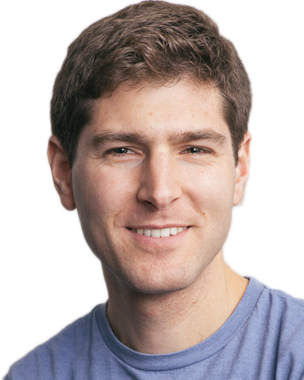
\includegraphics[width=1in,height=1.25in,clip,keepaspectratio]{photos/karr.jpg}}]{Jonathan R. Karr}
received his Ph.D. in Biophysics and M.S. in Medicine from Stanford University, USA in 2014 and his B.S.s in Physics and Brain \& Cognitive Sciences from the Massachusetts Institute of Technology, USA in 2006. Currently, Dr. Karr is a Fellow at the Icahn School of Medicine at Mount Sinai, USA. His research focuses on the development of comprehensive whole-cell computational models and their applications to bioengineering and medicine.
\end{IEEEbiography}

\begin{IEEEbiography}{Herbert M. Sauro}
Biography text here.
\end{IEEEbiography}

\end{document}